% ! TeX program = pdflatex

\documentclass{article}

\usepackage[a4paper, margin = 1in]{geometry}
\usepackage{listings}
\usepackage{color}
\usepackage{graphicx}
\usepackage{tikz}
\usepackage{dirtree}
\usepackage{hyperref}
\usepackage[maxbibnames=10]{biblatex}

\hypersetup{
	colorlinks=true,
	linkcolor=blue,
	filecolor=blue,
	urlcolor=blue,
	citecolor=blue,
}

\addbibresource{references.bib}

\newcommand{\code}[1]{\texttt{#1}}

\title
{
	CS420 Compiler Design\\
	Report for the Term Project: Final Report\\
	${}$\\
	Team 12
}

\author
{
	Jaeseong Choe\\
	Undergraduate\\
	Department of Physics, KAIST
	\and
	Kee Tack Kim\\
	Undergraduate\\
	Department of Mathematics, KAIST
	\and
	Taeyoung Kim\\
	Undergraduate\\
	School of Computing, KAIST
	\and
	Youngrae Kim\\
	Undergraduate\\
	School of Computing, KAIST
	\and
	Seokbin Lee\\
	Undergraduate\\
	School of Computing, KAIST
}

\begin{document}
	\maketitle
	
	\section{Introduction}
	
	\subsection{ARTIDE}
	
	We named our project by \emph{ARTIDE}. The word ARTIDE is an abbreviation for \emph{A Really Tiny Integrated Development Environment}. ARTIDE provide only compiler and debugger for the mini-C programming language. Since it does not provide other common options of IDE like source code editor and linker, it seem to deficiency to called by IDE. However, we choose this naming for the future development. In Italian, the word ARTIDE means the north pole of the earth. Hence, we choose polar bear as our trademark. The project ARTIDE implemented by using Python programming language.
	
	\begin{figure}
		\centering
		\includegraphics[width=0.6\textwidth]{"../img/polar bear 2".png}
		\caption{Polar bears.}
		\label{fig: polar bears}
	\end{figure}
	
	\subsection{Directory structure}
	
	Our project directory has the following structure:
	\dirtree{%
		.1 /.
		.2 /doc.
		.3 /doc/img.
		.3 /doc/tex.
		.3 Some documentations from TA.
		.3 Some documentations by ourselves.
		.2 /lib.
		.3 /lib/ply.
		.4 /lib/ply/lex.py.
		.4 /lib/ply/yac.py.
		.2 /src.
		.3 /src/lexical\_analyzer.py.
		.3 /src/syntax\_analyzer.py.
		.3 /src/semantic\_analyzer.py.
		.3 /src/intermediate\_code\_generator.py.
		.3 /src/code\_generator.py.
		.3 /src/debugger.py.
		.2 /test.
		.2 /.gitignore.
		.2 /LICENSE.
		.2 /README.md.
	}
	
	In the root directory \code{/}, there are four sub-directories \code{/doc} for store the documentation files, \code{/lib} for library files, \code{/src} for source code files, and \code{/test} for test code files. In the root directory, there are also some files that containing some information of the project. \code{/.gitignore} contains the ignore information for git, \code{/LICENSE} contains the license information of the project, and \code{/README.md} contains explanation about the project as the form of markup document.
	
	\subsection{Publication}
	
	We published our project as GitHub public repository with MIT License. You can check our source code and other information from \url{https://github.com/JaeseongChoe/KAIST-CS420-Term\_Project}.
	
	\section{mini-C specification}
	
	The mini-C programming language is an subset of the ANSI-C (C89/C90).\\
	The mini-C supports:
	\begin{itemize}
		\item Primitive data types:
		
		\code{int}, \code{float}, \code{double}, \code{char}, \code{str} $+$ \code{array} and \code{pointer} types for them
		
		\item Primitive operations:
		
		Arithmetic, comparison\&relation, logical, bitwise, and assignment operations.
	\end{itemize}
	The mini-C does not supports:
	\begin{itemize}
		\item Some complex data types:
		
		\code{struct}, \code{union}, and \code{enum} types.
		
		\item User defined data types.
		
		\item Type qualifiers:
		
		\code{signed}, \code{unsigned}, \code{const}, \code{volatile}, \code{static}, \code{auto}, and \code{register}.
	\end{itemize}
	
	\section{Libraries and modules}
	
	\subsection{PLY library}
	
	Lexical analyzer and syntax analyzer of the mini-C compiler in ARTIDE implemented by using PLY (Python Lex-Yacc) library (PLY-3.11). The PLY library has two modules \code{lex.py} and \code{yacc.py}. In the \code{lex.py} file, there is a special class for tokenization phase called \code{LexToken}. The class \code{LexToken} has four attributes:
	
	\begin{itemize}
		\item \code{self.type}
		
		\code{self.type} field represent the type of each token. For example, lexime \code{1234} has the token type \code{ICONST} after it tokenized.
		
		\item \code{self.value}
		
		\code{self.value} field represent the original string of each token. For example, lexime \code{1234} has the value \code{`1234'} after it tokenized.
		
		\item \code{self.linno}
		
		\code{self.lino} field represent the line number of each lexime in the source file.
		
		\item \code{self.lexpos}
		
		\code{self.lexpos} field represent the position of first charactor of each lexime relative to the start of source file.
	\end{itemize}
	
	Figure \ref{fig: tokenization} shows that how the tokenization phase works. If the lexical analyzer meet \code{var = 1234;} at line 10 of source file, then it produces the tokens like \code{\code{(ID, `var', 10, 53)}}, \code{(ASSIGN, `=', 10, 57)}, \code{(ICONST, `1234', 10, 59)}, and \code{(COLON, `:', 10, 63)} with predefined matching rules for each lexime.
	
	\begin{figure}[ht]
		\centering
		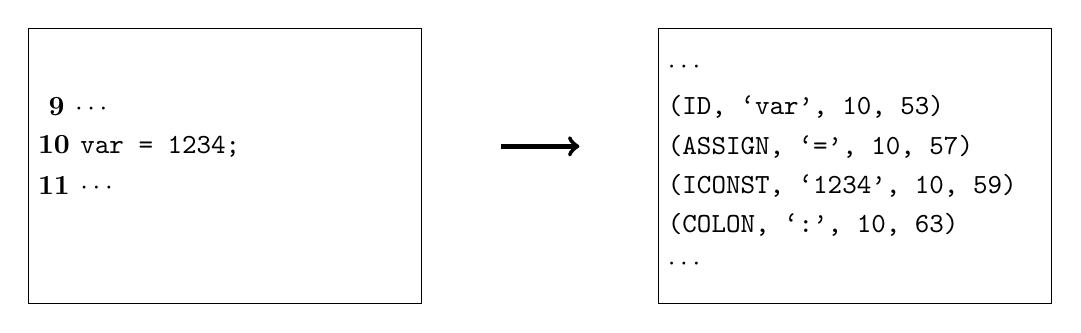
\begin{tikzpicture}
		\draw (0,3.5) rectangle (5,0);
		\draw (0,2.5) node[anchor=west] {\textbf{ 9 }\code{$\cdots$}};
		\draw (0,2.0) node[anchor=west] {\textbf{10 }\code{var = 1234;}};
		\draw (0,1.5) node[anchor=west] {\textbf{11 }\code{$\cdots$}};
		
		\draw[->, ultra thick] (6,2) -- (7,2);
		
		\draw (8,3.5) rectangle (13, 0);
		\draw (8,3.0) node[anchor=west] {\code{$\cdots$}};
		\draw (8,2.5) node[anchor=west] {\code{(ID, `var', 10, 53)}};
		\draw (8,2.0) node[anchor=west] {\code{(ASSIGN, `=', 10, 57)}};
		\draw (8,1.5) node[anchor=west] {\code{(ICONST, `1234', 10, 59)}};
		\draw (8,1.0) node[anchor=west] {\code{(COLON, `:', 10, 63)}};
		\draw (8,0.5) node[anchor=west] {\code{$\cdots$}};
		\end{tikzpicture}
		\caption{Tokenization.}
		\label{fig: tokenization}
	\end{figure}
	
	\subsection{\code{node.py} module}
	
	The \code{node.py} module is an our own module for constructing the abstract syntax tree of the input \code{.c} file. There is only one class called \code{Node} in this module and it has the following attribute:
	
	\begin{itemize}
		\item \code{self.type}
		
		The field \code{self.type} represent the type of the node. This type information may can be \code{INT}, \code{CHAR}, \code{If}, \code{IfElse}, \code{While}, and \code{For}.
		
		\item \code{self.value}
		
		The field \code{self.value} represent the label of the node. It can be operator like \code{+} and \code{-} for some expression statement.
		
		\item \code{self.lineno}
		
		The field \code{self.lineno} represent the line number of the statement in the original input \code{.c} file.
		
		\item \code{self.children}
		
		The field \code{self.children} represent the list of child nodes.
	\end{itemize}
	
	\subsection{\code{ast.py} module}
	
	The \code{ast.py} module is an our own module for construction the abstract syntax tree of the input \code{.c} file with another scheme. In \code{ast.py} module, there are many class with can be divide into three groups. The first group for defining type information, the second group for abstract syntax information of the operators, and the third group for defining various types of node in abstract syntax tree.
	
	The first group has only one class \code{Type(enum.Enum)}. It defines the type information like \code{Type.VOID}, \code{Type.INT}, \code{Type.FLOAT}, \code{Type.CHAR}. This type information used for translation from concrete syntax to abstract syntax, and implementation of the type checker.
	
	The second group has classes that define the abstract syntax information of operators. The role of it is removing ambiguity in the concrete syntax. For example, the token \code{+} in concrete syntax can be has two different semantic, namely, binary addition operator \code{+} (eg. \code{x + y}) and unary sign operator \code{+} (eg. \code{+3.14}). The second group has the following list of classes \code{Operator(enum.Enum)}, \code{ArithOp(enum.Enum)}, \code{ComRelOp(enum.Enum)}, \code{LogicalOp(enum.Enum)}, \code{BitwiseOp(enum.Enum)}, \code{AssignOp(enum.Enum)}, and \code{MemPoinOp(enum.Enum)}.
	
	The third group has classes that define various types of node in abstract syntax tree. It contains \code{Node(object)}, \code{ID(Node)}, \code{Subscript(Node)}, \code{FunCall(Node)}, \code{Args(Node)}, \code{UnaOp(Node)}, \code{BinOp(Node)}, \code{TerOp(Node)}, \code{Assign(Node)}, \code{Expr(Node)}, \code{If(Node)}, \code{IfElse(Node)}, \code{Switch(Node)}, \code{Case(Node)}, etc.
	
	\subsection{\code{symtab.py} module}
	
	The \code{symtab.py} module is an our own module for construct the symbol table and funtion table. It implemented by using the dictionary which is the one of Python built-in data type to provide hash table feature. Our symbol table structure has the hierarchy as shown in Figure \ref{fig: hierarchy of symbol table} by its scope (or block). In order to implement this hierarchy, we define the two classes \code{SymTabBlock} and \code{SymTab}. The class \code{SymTabBlock} represents a symbol table for certain block, and \code{SymTab} represents and manages a overall hierarchy of these blockwise symbol tables.
	
	\begin{figure}[ht]
		\centering
		\includegraphics[width=0.55\textwidth]{"../img/symbol table hierarchy".png}
		\caption{The hierarchy of symbol table. \cite{Aho:2006:CPT:1177220}}
		\label{fig: hierarchy of symbol table}
	\end{figure}
	
	Furthermore, there is one another class for collecting the data about certain symbol (or identifier) called \code{SymTabEntry}. The class \code{SymTabEntry} has three attributes:
	
	\begin{itemize}
		\item \code{self.id}
		
		\code{self.id} field represents the identifier as a string.
		
		\item \code{self.type}
		
		\code{self.type} field represents the type of that identifier. For example, if the identifier \code{var} declared in source file with the type \code{int}, then \code{self.type} of \code{SymTabEntry} for this identifier is \code{INT}.
		
		\item \code{self.assigned}
		
		\code{self.assigned} field represents the weather some value was assigned to that identifier or not by boolean (\code{True} or \code{False}).
	\end{itemize}
	
	\code{SymTabBlock} is a symbol table of each block. The class \code{SymTabBlock} has three attributes:
	
	\begin{itemize}
		\item \code{self.prev}
		
		\code{self.prev} field represents the symbol table of the direct outer block of current block. For example, in the case of Figure \ref{fig: hierarchy of symbol table}, \code{self.prev} of $B_1$ pointing to $B_0$.
		
		\item \code{self.nexts}
		
		\code{self.nexts} field represent the list of symbol tables for the direct inner blocks of current block. For example, in the case of Figure \ref{fig: hierarchy of symbol table}, \code{self.nexts} of $B_1$ is a list \code{[$B_2$, \dots]}.
		
		\item \code{self.table}
		
		\code{self.table} is an actual table to save the information about each symbols. It is a dictionary object which is a builtin hash table object in Python. Hence, it corresponds to table in the right side of each labels in Figure \ref{fig: hierarchy of symbol table}.
	\end{itemize}
	
	\code{SymTab} is a management system for overall collection of \code{SymTabBlock}. The class \code{SymTab} has one attribute and five methods:
	
	\begin{itemize}
		\item \code{self.cur}
		
		\code{self.cur} pointing to the current symbol table.
		
		\item \code{insert\_block\_table(self, block\_table)}
		
		\code{insert\_block\_table} method provides feature that insert new symbol table into the management system. It appends the \code{block\_table} into the list \code{self.nexts} of the current symbol table. Then, it changes \code{self.cur} to \code{block\_table}.
		
		\item \code{remove\_block\_table(self)}
		
		\code{remove\_block\_table} method provides feature that remove the current symbol table. It pops the current symbol table from the list \code{self.nexts} of symbol table for direct outer block. Then, it changes \code{self.cur} to symbol table for direct outer block. 
		
		\item \code{insert(self, symbol)}
		
		\code{insert} method provides a feature that register the information of new symbol into current symbol table. The input parameter \code{symbol} is a \code{SymTabEntry} object. \code{insert} method check that there already exist a symbol with same identifier with the input parameter \code{symbol}. If there is no such a symbol, then \code{insert} registers the \code{symbol} into current symbol table with setting the hash key as its identifier \code{symbol.id}. If there is such a symbol, \code{insert} produces an error \code{DupDeclError}.
		
		\item \code{remove(self, id)}
		
		\code{remove} method provides a feature that deregister the information about identifier \code{id} from the current symbol table. \code{remove} check weather there exist the information about that identifier. If there is such information, then it removes the hash information of that identifier. If there no such information, then it produces an error \code{UndefIdError}.
		
		\item \code{get(self, id)}
		
		\code{get} method provides a feature that searching the information about identifier \code{id}. \code{get} searches the information with the manner of starting from current symbol table to outer symbol tables. If \code{get} succeed to find that information, then it returns that information as the form of \code{SymTabEntry}. If \code{get} failed to find that information, then it produces an error \code{UndefIdError}.
	\end{itemize}
	
	Figure \ref{fig: illustration of the hierarchy of symbol table classes} illustrates the hierarchy of symbol table. The outermost rectangle of blue color represents the symbol table management class \code{SymTab}. An arrow represents the \code{self.cur} attribute of \code{SymTab}. The rest rectangles of gray color represent the symbol tables class \code{SymTabBlock} for each blocks.
	
	\begin{figure}[ht]
		\centering
		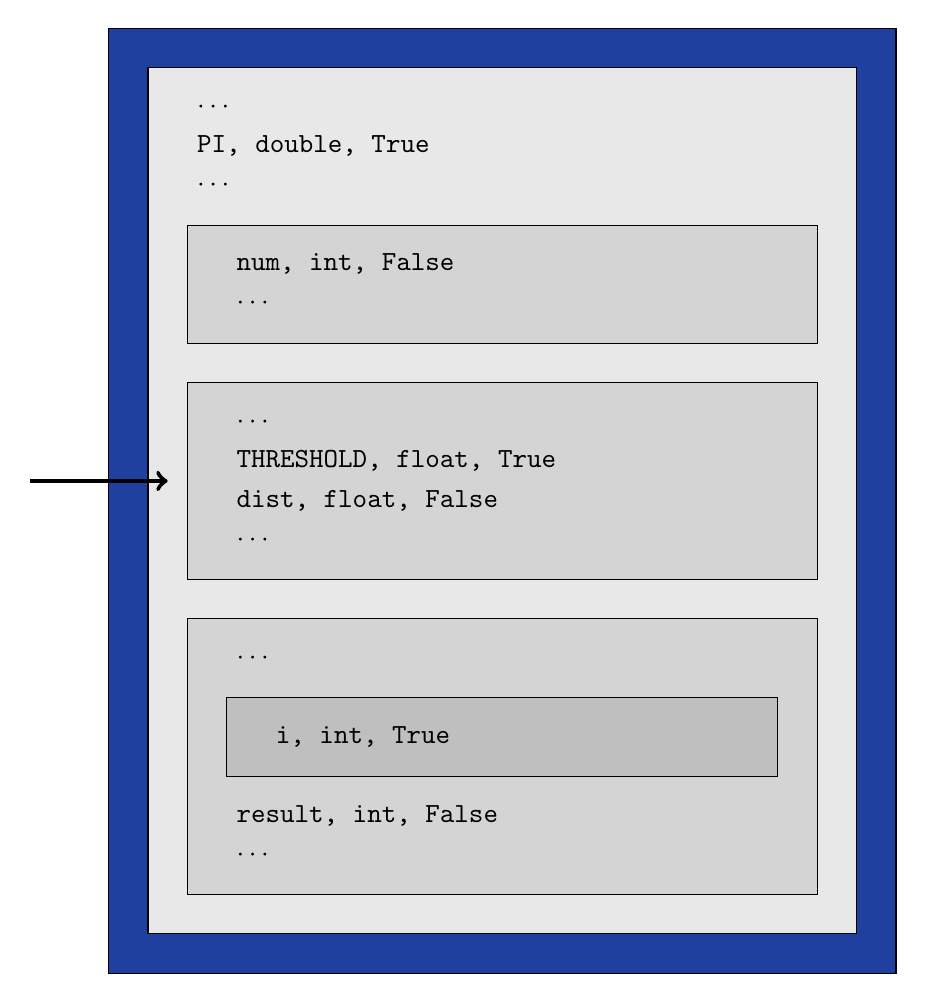
\begin{tikzpicture}
		\draw[fill={rgb:red,1;green,2;blue,5}] (0,0) rectangle (10, 12);
		
		\draw[fill={rgb:black,1;white,10}] (0.5,0.5) rectangle (9.5, 11.5);
		
		\draw[fill={rgb:black,1;white,5}] (1,1) rectangle (9, 4.5);
		\draw[fill={rgb:black,1;white,5}] (1,5) rectangle (9, 7.5);
		\draw[fill={rgb:black,1;white,5}] (1,8) rectangle (9, 9.5);
		
		\draw[fill={rgb:black,1;white,3}] (1.5,2.5) rectangle (8.5, 3.5);
		
		
		\draw (1,11) node[anchor=west] {\code{$\cdots$}};
		\draw (1,10.5) node[anchor=west] {\code{PI, double, True}};
		\draw (1,10) node[anchor=west] {\code{$\cdots$}};
		
		\draw (1.5,9) node[anchor=west] {\code{num, int, False}};
		\draw (1.5,8.5) node[anchor=west] {\code{$\cdots$}};
		
		\draw (1.5,7) node[anchor=west] {\code{$\cdots$}};
		\draw (1.5,6.5) node[anchor=west] {\code{THRESHOLD, float, True}};
		\draw (1.5,6) node[anchor=west] {\code{dist, float, False}};
		\draw (1.5,5.5) node[anchor=west] {\code{$\cdots$}};
		
		\draw (1.5,4) node[anchor=west] {\code{$\cdots$}};
		\draw (2,3) node[anchor=west] {\code{i, int, True}};
		\draw (1.5,2) node[anchor=west] {\code{result, int, False}};
		\draw (1.5,1.5) node[anchor=west] {\code{$\cdots$}};
		
		
		\draw[->, ultra thick] (-1,6.25) -- (0.75,6.25);
		\end{tikzpicture}
		\caption{Illustration of the hierarchy of symbol table classes.}
		\label{fig: illustration of the hierarchy of symbol table classes}
	\end{figure}
	
	\section{mini-C compiler}
	
	The mini-C compiler in ARTIDE has three different parts, namely, front end, middle end, and back end. The front end consist of three phases lexical, syntax, and semantic analysis. The middle end and back end both consist of only one phase intermediate code generation and code generation, respectively.
	
	\subsection{Lexical analyzer}
	
	The lexical analyzer uses \code{lex.py} module of the PLY library. Token specification of mini-C can be found in \code{/src/lexical\_analyzer.py}. It can covers all the tokens of ANSI-C (C89/C90).
	
	\subsection{Syntax analyzer}
	
	The syntax analyzer uses \code{yacc.py} module of the PLY library. Context sensitive grammar within BNF can be found in \code{/src/syntax\_analyzer.py}. The parsing mechnism of generated syntax analyzer is LALR(1).
	
	\subsection{Semantic analyzer}
	
	The semantic analyzer of the mini-C compiler in ARTIDE provides three different feature.
	
	\begin{itemize}
		\item Construction of the symbol table and the function table.
		
		\item Static checking
		
		\begin{itemize}
			\item While the constructing the symbol table and the function table, it check the existence of undeclared or duplicated identifier error.
			
			\item It also check that weather the \code{continue} and \code{break} statement are located inside loop or not.
		\end{itemize}
		
		\item Type checking
		
		\begin{itemize}
			\item Check the types of operands for arithmetic operators.
			\item Check the types of destination and source element in assignment statement.
			\item While the type checking phase, insert the proper type casting operation when it need to and possible to match the types of operands. 
		\end{itemize}
	\end{itemize}
	
	\subsection{Intermediate code generator}
	
	The intermediate code generator get the abstract syntax tree as its input and returns the string of intermediate code as its output. The form of intermediate code is the \emph{three address code}.	
	
	\subsection{Code generator}
	
	The code generator get the string of intermediate code as its input and returns the string of assembly code for the x86 architecture with AT\&T syntax.
	
	\section{mini-C debugger}
	
	The mini-C debugger in ARTIDE provide two different features, namely, interpreting feature and debugging feature.
	
	\subsection{Interpreting feature}
	
	Interpreting feature provides the way that interpret the input \code{.c} file as line by line. There are only one command to control the interpreting feature.
	
	\begin{itemize}
		\item \code{next}
		
		The command \code{next} excutes a single or multiple lines(s) of the source code. For example. \code{next} just excutes current line of source code, and \code{next 10} will excute 10 lines including current line.
	\end{itemize}
	
	\subsection{debugging feature}
	
	Debugging feature provides the helpful options for debug the input \code{.c} file. There are two commands to control the debugging feature.
	
	\begin{itemize}
		\item \code{print}
		
		The command \code{print} provides feature that print the value contained in a variable at the moment. For example, if an integer variable \code{x} contains value \code{10}, then \code{print x} will print \code{10}.
		
		\item \code{trace}
		
		The command \code{trace} provides feature that trace the history of a variable from the beginning to the moment.
	\end{itemize}
	
	\nocite{*}
	\printbibliography
\end{document}